%!TEX root = ../thesis.tex

\chapter{Methods}
\label{cha:methods}

In this chapter we are going to explained the different methods used during this thesis.
First we are going to explained the backbone architecture used during the whole thesis.
Then we are going to explain how we performed a model to track points.
The last section will explain how metric learning works and how we have use it.

\section{Backbone Architecture}
\label{sec:methods_backbone_architecture}

The objective of this thesis has been to obtain a deep learning model which is capable of given a point per instance, be able to predict its segmentation through all the videos.
As it is usual on the literature, the best deep learning models for computer vision tasks (and more concretly in segmentation) are the ones that are fully convolutional neural networks.
This models perform convolution operations over the input which is commonly an image.

During the development of this thesis, we have used as a backbone architecture the DeepLab~\cite{chen2018deeplab} model used for semantic segmentation.
This model is a fully convolutional model based on the ResNet~\cite{he2016deep} architecture which was used for image classification.
The DeepLab~\cite{chen2018deeplab} model what does is to keep the convolutional layers from ResNet~\cite{he2016deep} and add at the end some deconvolutional operatons to obtain as an output a mask instead of an object classifier.
Doing this allows to be the model fully convolutional and free the constrain about the input images size's.

The ResNet architecture are based on layers with residual connections. In \figref{resnet_block} is showed how each bottleneck layer block is build, which is the mainly used.
Each layer apply some convolutional operations to the input and then add this result to the original input as a residual.

\begin{figure}[h]
  \centering
  \adjincludegraphics[trim={{.5\width} 0 0 0}, clip, width=.5\textwidth]{figures/resnet/block_deeper.pdf}
  \caption{ResNet residual block architecture. }
  \label{fig:resnet_block}
\end{figure}

To check out the whole architecture of the DeepLab convolutional neural network see \tabref{deeplab_arch} where the whole architecture is explained for the two versions used: ResNet50 and ResNet101.
The architecture is taking as input images of size $512 \times 512$ and outputing this size downsampled by $8$ both in height and width. Also note that output number of channels are 2048, so this output can be used, or a header can be pluged to reduce the dimensionality or build a classifier to obtain a mask.
Because of these, this architecture is very versatile and easy to use with images.

\newcommand{\blocka}[2]{\multirow{3}{*}{\(\left[\begin{array}{c}\text{3$\times$3, #1}\\[-.1em] \text{3$\times$3, #1} \end{array}\right]\)$\times$#2}
}
\newcommand{\blockb}[3]{\multirow{3}{*}{\(\left[\begin{array}{c}\text{1$\times$1, #2}\\[-.1em] \text{3$\times$3, #2}\\[-.1em] \text{1$\times$1, #1}\end{array}\right]\)$\times$#3}
}
\begin{table}[h]
  \centering
  \begin{tabular}{c|c|c|c}
    \toprule
    layer name & output size & 50-layer & 101-layer \\
    \midrule
    conv1 & 256$\times$256 & \multicolumn{2}{c}{7$\times$7, 64, stride 2}\\
    \midrule
    \multirow{4}{*}{conv2\_x} & \multirow{4}{*}{128$\times$128} & \multicolumn{2}{c}{3$\times$3 max pool, stride 2} \\\cline{3-4}
      &  &  \blockb{256}{64}{3} & \blockb{256}{64}{3} \\
      &  &  &\\
      &  &  &\\
    \hline
    \multirow{3}{*}{conv3\_x} &  \multirow{3}{*}{64$\times$64}    & \blockb{512}{128}{4}  & \blockb{512}{128}{4}\\
      &  &  &\\
      &  &  & \\
    \hline
    \multirow{3}{*}{conv4\_x} & \multirow{3}{*}{64$\times$64}  & \blockb{1024}{256}{6}  & \blockb{1024}{256}{23} \\
      &  &  &\\
      &  &  & \\
    \hline
    \multirow{3}{*}{conv5\_x} & \multirow{3}{*}{64$\times$64}  &  \blockb{2048}{512}{3}  & \blockb{2048}{512}{3}\\
      &  &  &\\
      &  &  & \\
    \bottomrule
  \end{tabular}
  \caption{Architectures for DeepLab using residual blocks.
    Building blocks are shown in brackets (see also \figref{resnet_block}), with the numbers of blocks stacked.
  }
  \label{tab:deeplab_arch}
\end{table}


\section{Tracking}
\label{sec:methods_tracking}

In order to track points through a video sequence, one approach we have tested consisted on regress the point position in an image usng a heatmap.
The point representation is inspired by~\cite{nam2016learning} which used heatmaps to predict keypoints positions.
In our experiments we are going to use the DeepLab ResNet architecture described in Section~\ref{sec:methods_backbone_architecture} plus an additional module, a PSP~\cite{zhao2017pyramid} module that will reduce the last layer channels to a single channel using a pyramid scene parsing.
This will allow us to regress a heatmap representation of a point using Mean Sequared Error loss.

The heatmap is build given a point coordinates $p = (p_x, p_y)$ and computing a guassian arround this point.
In \equref{heatmap} is shown how to build a heatmap $\mathcal{H}$ which allows some customization with the chosing of the parameter $\sigma$ which is the spreadness of the sigma.
Note that the values of the heatmap are bounded between $[0, 1]$.
To observe a graphical example, in \figref{point_representation} there is a point annotated on an image and the resulting heatmap.

\begin{equation}
  \mathcal{H}(x, y) = \exp \left[ -4 \log(2) \frac{ (x - p_x)^2 + (y - p_y)^2 }{ \sigma^2 } \right]
  \label{eq:heatmap}
\end{equation}

\begin{figure}[h]
  \centering
  \begin{subfigure}{.5\textwidth}
    \centering
    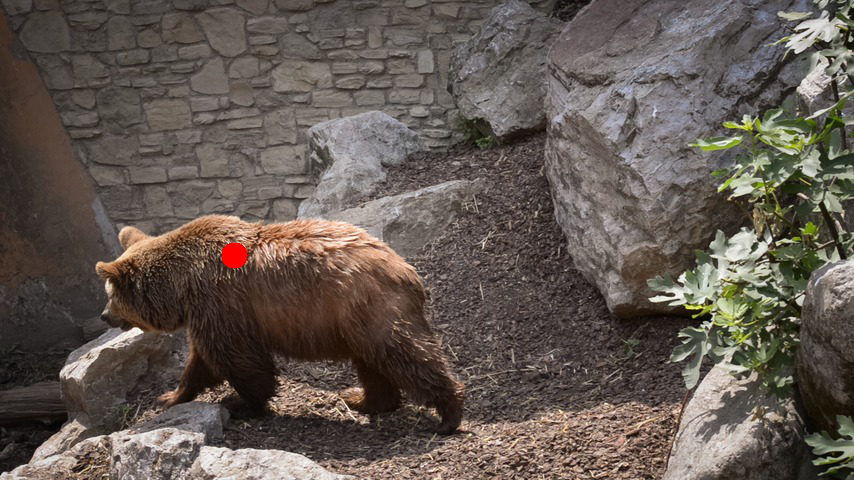
\includegraphics[width=.8\linewidth]{figures/methods/heatmaps/image_point.png}
  \end{subfigure}%
  \begin{subfigure}{.5\textwidth}
    \centering
    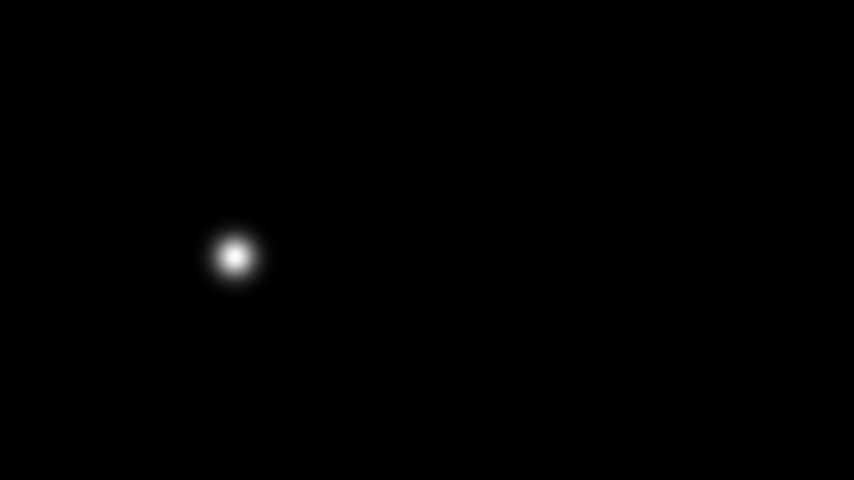
\includegraphics[width=.8\linewidth]{figures/methods/heatmaps/heatmap.png}
  \end{subfigure}
  \caption{
  Point representation.
  \textbf{Left}. Image with the annotated points (image resolution $854 \times 480$ pixels).
  \textbf{Right}. Heatmap to represent the point with $\sigma = 32$ pixels. }
  \label{fig:point_representation}
\end{figure}

The strategy to train a model that tracks a point given in the first frame will be the same as in the OSVOS~\cite{caelles2017one} approach.
We will finetune a model pretrained with Visual Object Classes over the first frame of each sequence.
Adding some data augmentation to enrich the training, we will test each sequence models with the rest of the frames and extract the maximum of the predicted heatmap as tracked object.

\section{Metric Learning with Triplet Loss}
\label{sec:methods_metriclearning}

Another method we have tried during the devleopment of this thesis consist on train a model which outputs an embedding for each pixel that can be meaningfull to obtain an instance segmentation.
In order to obtain a good embedding, metric learning has been used which consists on the task of learning a distance function over objects, which in our case are embeddings.

One way to apply metric learning is using the Triplet Loss which was first introduced in~\cite{balntas2016learning}.
One famous implementation of this Triplet Loss was used in FaceNet~\cite{schroff2015facenet} where they train a model to embed face images and predict similarity between them.

The objective of the triplet loss consists on learning a distance difference between triplets of points.
The triplet consists on three points that are called: anchor, positive and negative.
It must fill the condition that the label of the anchor and the positive point are the same, while the label of the negative is different.
so what the triplet loss do is to push the distance of the anchor and positive points to be closer than the distance between the anchor and negative by some margin $\alpha$.
On \figref{triplet_loss_viz} there is a diagram about the learning procedure.

\begin{figure}[h]
  \centering
  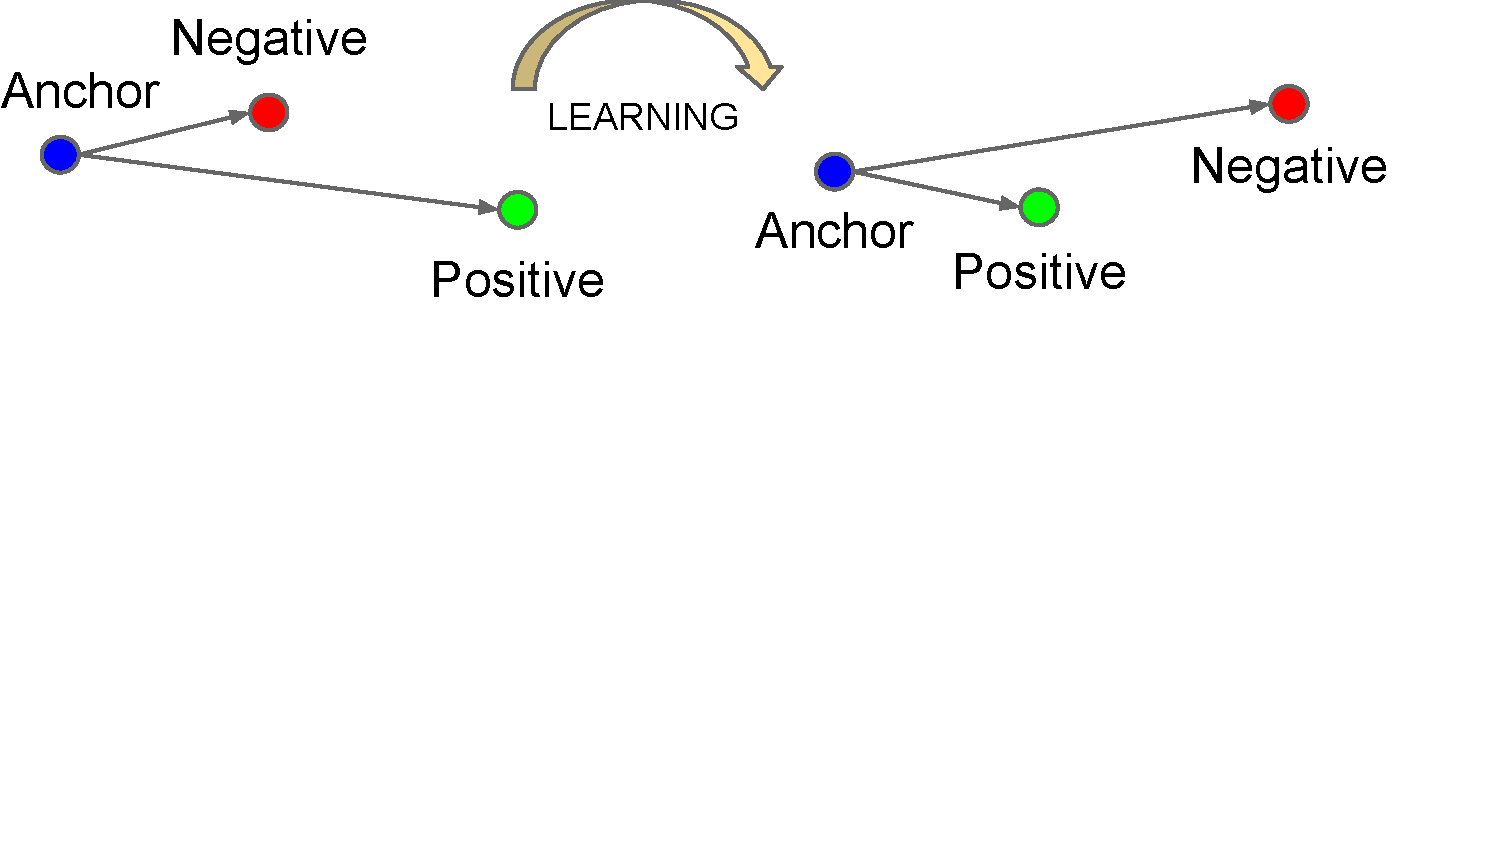
\includegraphics[trim=1cm 10cm 2.5cm 0cm, width=0.7\linewidth]{figures/methods/triplet_loss/triplet_viz.pdf}
  \caption{
    Graphical representation of Triplet Loss learning.
    Figure extracted from~\cite{schroff2015facenet}. }
  \label{fig:triplet_loss_viz}
\end{figure}

% TODO: This paragraph on previous section
In our escenario, we used an embedding model which is a the DeepLab~\cite{chen2018deeplab} explained in detail in Section~\ref{sec:methods_backbone_architecture}.
This model has been pretrained with semantic semgnetion from images, and we are using the full network except the last classification part which predicts the pixels class.
By default this model given an image of size $H \times W$ output a features map of size $H' \times W' = \frac{H}{8} \times \frac{W}{8}$ with $2048$ dimensions.
A convolutional head can be plugged to reduce this dimensionality to a lower dimension $D$ which may lead to a better embedding.

Before giving the equations of the Triple Loss, lets define some notation.
Be $\mathcal{I} \in \mathbb{R}^{H \times W}$ the input image of size $H \times W$.
The output size of the model will be $H' \times W' = \frac{H}{8} \times \frac{W}{8}$ and the output embedding will be $\mathcal{X} = \{x_i\}^{H' \times W'}$ where $x_i \in \mathbb{R}^D$ is the i-th output pixel embedding.
Lets be the Convolutional Neural Network as embedding model $f(\mathcal{I}; \Theta)$ which computes the embedding from a single image:

\begin{equation}
  \mathcal{X} = f(\mathcal{I}; \Theta)
\end{equation}

When training the model, there is available the ground truth mask of one object instance in the image. When the image is forwarded throught the model and the embeddings computed, $N$ triplets of pixels are sampled. For each triplet, two pixels with a mask set to 1 are sampled and assigned as anchor and positive pixels ($x_a$ and $x_p$ respectively). Finally a pixel with a mask set to 0 is sampled and assigened as negative pixel $x_n$.

\begin{equation}
  \label{eq:triplet_loss_1}
  \mathcal{L}_{triplet} = \sum_i^N \max \left( d(x_a^{(i)}, x_p^{(i)}) - d(x_a^{(i)}, x_n^{(i)})  + \alpha, 0 \right)
\end{equation}

The $\alpha$ term on the triplet loss is the margin used to inforce the minimum diference between the distance of positive pairs and negative pairs. $d$ is the distance function, which in our case the $l^2$ norm is used. So \equref{triplet_loss_1} will end up as follows:

\begin{equation}
  \label{eq:triplet_loss_2}
  \mathcal{L}_{triplet} =
	\sum_i^N \max \left(
		\|x_a^{(i)} - x_p^{(i)}\|_2 - \|x_a^{(i)} - x_n^{(i)}\|_2  + \alpha,
		0 \right)
\end{equation}

This learned embedding can be very useful for example to implement a second approach for tracking.
A similarity between pixel's embedding in the next frame and the embedding of the point to track in order to obtain its location on the next frame.


% TODO:
% At some point we tried to implement 2 triplet loss.
% Explain the precedure for far/close pixels.

\section{Embedding Segmentation}

Once we have learned a good embedding for each pixel of the image, the embedding can not gives us directly the segmentation of every instance.
As our approach will consists on track a point for every instance in the video sequence, an already annotated pixel will be provided.
This pixel which we will know already its label we are going to call it keypoint with an embedding $x_k \in \mathbb{R}^D$ and this point can be point comming from the ground truth, from tracking or from another frame annotation.

In order to obtain the segmentation for multiple instances on the images given a keypoint of instance can be done computing the distance of every pixel embedding against all keypoint's embeddings.
Then every pixel will be assigned to the label of the closest keypoint embedding only if this distance is lower than a threshold $\gamma$, otherwise will be assign as background.
All of this can be formulated mathematically taking into account and image embedding $\mathcal{X} = {x_i}^{H \times W}$ with $N$ instances and each instance with a keypoint embedding $x_k^{(n)}$.
Every keypoint will have a label $m_k^{(n)} \in [1, N]$ and label $0$ will belong to the background.
The distance map for every image will be:

\begin{equation}
  \mathcal{D}_i = min_n \left( d(x_i, x_k^{(n)}) \right)
\end{equation}

Then the prediction label can be computed as follows:

\begin{equation}
  \mathcal{M}_i = \begin{cases}
      \arg\min_n d(x_i, x_k^{(n)}) & \mathcal{D}_i \leq \gamma \\
      0 & \mathcal{D}_i > \gamma
   \end{cases}
\end{equation}

All this steps can be visualize on an example image in \figref{instance_segmentation} where are displayed the ground truth mask and a keypoint per each dog instance, the distance map of the embeddings agains the keypoint embedding and finally the predicted mask.

\begin{figure}[h]
  \centering
  \instancesegmentation{1}
  \instancesegmentation{2}
  \instancesegmentation{3}
  \caption{Example of instance segmentation procedure given a point per instance.
  \textbf{Left} Ground truth annotation of the instance and keypoint given.
  \textbf{Middle} Distance map of the every pixel's embedding versus keypoint embedding (higher intensisy means lower distance, dark means higher distance).
  \textbf{Right} Predicted mask once applied the thresholding. }
  \label{fig:instance_segmentation}
\end{figure}
